\begin{blocksection}
\question Draw the environment diagram that results from running the following code.
\begin{lstlisting}
ghost = [1, 0,[3], 1]
def boo(spooky):
  ghost.append(spooky.append(ghost))
  spooky = spooky[ghost[2][1][1]]
  ghost[:].extend([spooky])
  spooky = [spooky] + [ghost[spooky - 1].pop()] 
  ghost.remove(ghost.remove(1))
  spooky += ["Happy Halloween!"]
  return spooky
pumpkin = boo(ghost[2])
\end{lstlisting}

\begin{solution}[1in]
  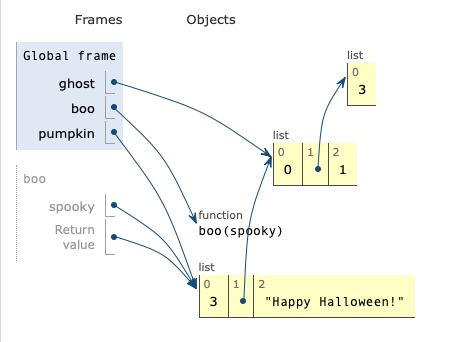
\includegraphics[width=.5\textwidth]{spooky-list_sol.png}
  \newline
  \href{http://pythontutor.com/visualize.html#code=ghost%20%3D%20%5B1,%200,%5B3%5D,%201%5D%0Adef%20boo%28spooky%29%3A%0A%20%20%20%20%20%20%20%20ghost.append%28spooky.append%28ghost%29%29%0A%20%20%20%20%20%20%20%20spooky%20%3D%20spooky%5Bghost%5B2%5D%5B1%5D%5B1%5D%5D%0A%20%20%20%20%20%20%20%20ghost%5B%3A%5D.extend%28%5Bspooky%5D%29%0A%20%20%20%20%20%20%20%20spooky%20%3D%20%5Bspooky%5D%20%2B%20%5Bghost%5Bspooky%20-%201%5D.pop%28%29%5D%20%0A%20%20%20%20%20%20%20%20ghost.remove%28ghost.remove%281%29%29%0A%20%20%20%20%20%20%20%20spooky%20%2B%3D%20%5B%22Happy%20Halloween!%22%5D%0A%20%20%20%20%20%20%20%20return%20spooky%0A%20%20%20%20%20%20%20%20%0Apumpkin%20%3D%20boo%28ghost%5B2%5D%29&cumulative=false&heapPrimitives=nevernest&mode=edit&origin=opt-frontend.js&py=3&rawInputLstJSON=%5B%5D&textReferences=false}{PythonTutor Link} 
\end{solution}
\begin{guide}
\textbf{Teaching Tips}
\newline
  Explanations for some tricky steps:
  \begin{itemize}
    \item Line 3: \lstinline{append} returns \lstinline{None}, so \lstinline{ghost} is appended to \lstinline{spooky} and \lstinline{None} is appended to \lstinline{ghost}
    \item Line 5: This does nothing because the value of this expression is never assigned to a variable. List slicing creates a copy of a list that is immediately deleted
    \item Line 6: Pop returns the last element of the original value of spooky. Since we use \lstinline{=} and then \lstinline{+} instead of \lstinline{+=}, a new list is created
    \item Line 7: \lstinline{remove} deletes the first element with a given value, so the first instance of 1 is deleted. \lstinline{remove} returns \lstinline{None}, so the outer call to \lstinline{remove} gets rid of the \lstinline{None} element of \lstinline{ghost}
    \item Line 8: \lstinline{+=} mutates \lstinline{spooky} instead of creating a new list 

  \end{itemize}
\end{guide}
\end{blocksection}